\chapter{Chocs de particules}

\section{D\'esint\'egration des particules}

Les lois de conservations ne d\'ependent absolument pas de l'esp\`ece d'interaction entre les particules et permettent ainsi d'arriver \`a des conclusions pourtant importantes pour les processus m\'ecaniques en jeu.

Pour commencer, choisissons la d\'esint\'egration spontan\'ee, i.e. non provoqu\'ee par des forces ext\'erieures, d'une particule en deux autres particules se d\'epla\c{c}ant apr\`es la d\'esint\'egration ind\'ependamment l'une de l'autre. Sa forme la plus simple est quand il est consid\'er\'e dans un syst\`eme de r\'ef\'erence o\`u la particule initiale est au repos. La conservation d' l'impulsions implique :
\bea
	\vec{p}_{1} + \vec{p}_{2} & = & \vec{0} \nonumber \\
	\vec{p}_{1} & = & -\vec{p}_{2}
\eea
ainsi les particules r\'esultantes de la d\'esint\'egration s'\'eloignent l'une de l'autre avec des impulsions \'egales, ,$\lVert \vec{p}_{1} \rVert = \lVert \vec{p}_{2} \rVert = p_{0}$ et dirig\'ees en sens inverse.

En utilisant la loi de conservation de l'\'energie et en particulier l'\'equation (\ref{EQ:8_4}) et parce que l'\'energie cin\'etique de la particule initiale est nulle, nous pouvons \'ecrire :
\be
	E_{int} = E_{1int} + \dfrac{p_{0}^{2}}{2m_{1}} + E_{2int} + \dfrac{p_{0}^{2}}{2m_{2}}
\ee
avec $E_{int}$ l'\'energie interne de la particule initiale, $E_{1int}$ et $E_{2int}$ l'\'energie interne des deux particules cr\'e\'ees. En d\'efinissant l'\'energie de d\'esint\'egration $\epsilon$ telle que :
\be
	\epsilon = E_{int} - (E_{1int} + E_{2int}) \label{EQ:16_1}
\ee
sa valeur est de facto positive. Or :
\be
	E_{int} - (E_{1int} + E_{2int}) = p_{0}^{2}\left(\dfrac{1}{2m_{1}} + \dfrac{1}{2m_{2}}\right)
\ee
Donc :
\be
	\epsilon = p_{0}^{2}\left(\dfrac{1}{2m_{1}} + \dfrac{1}{2m_{2}}\right) = \dfrac{p_{0}^{2}}{2m} \label{EQ:16_2}
\ee
avec $m = \dfrac{m_{1} + m_{2}}{m_{1}m_{2}}$ qui est la masse r\'eduite du syst\`eme apr\`es d\'esint\'egration.

\begin{figure}[htb!]
	\begin{center}
		\begin{picture}(500,300)(0,0)
			%circles
			\linethickness{0.05mm}
			\put(100,150){\circle{200}}\put(90,25){$V < v_{0}$}
			\put(400,150){\circle{200}}\put(390,25){$V > v_{0}$}
			%vectors circle #1
			\linethickness{0.5mm}
			\put(40,150){\vector(1,0){60}}\put(65,135){$\vec{V}$}
			\put(100,150){\vector(1,1){72}}\put(140,180){$\vec{v}_{0}$}
			\put(40,150){\vector(9,5){130}}\put(90,185){$\vec{v}$}
			%angles circle #1
			\linethickness{0.05mm}
			\qbezier(55,150)(55,155)(50,155)\put(60,152){$\theta$}
			\qbezier(110,150)(110,155)(105,155)\put(112,153){$\theta_{0}$}
			\multiput(100,150)(10,0){10}{\line(1,0){8}}
			%points circle #1
			\put(30,147){$A$}
			%vectors circle #2
			\linethickness{0.5mm}
			\put(250,150){\vector(1,0){150}}\put(320,135){$\vec{V}$}
			\put(400,150){\vector(1,1){72}}\put(440,180){$\vec{v}_{0}$}
			\put(250,150){\vector(10,3){220}}\put(390,210){$\vec{v}$}
			%\theta_{max} case
			\linethickness{0.05mm}
			\put(250,150){\line(10,9){90}}
			\put(400,150){\line(-11,15){60}}
			%angles circle #2
			\linethickness{0.05mm}
			\qbezier(280,150)(280,158)(275,158)\put(287,152){$\theta$}
			\qbezier(410,150)(410,155)(405,155)\put(412,153){$\theta_{0}$}
			\qbezier(320,150)(320,190)(294,190)\put(315,182){$\theta_{max}$}
			\multiput(400,150)(10,0){10}{\line(1,0){8}}
			%points circle #2
			\put(240,147){$A$}
			\put(300,155){$B$}
			\put(475,220){$C$}
		\end{picture}
		\caption{Repr\'esentation g\'eom\'etrique de d\'esint\'egrations}\label{FIG:4_14}
	\end{center}
\end{figure}

\'Etudions maintenant le cas o\`u la particule initiale poss\`ede une vitesse $\vec{V}$ non nulle avant la d\'esint\'egration dans le syst\`eme de r\'ef\'erence. Il en existe deux :
\begin{itemize}
	\item le syst\`eme du laboratoire ou <<~l~>>,
	\item le syst\`eme du centre d'inertie ou <<~c~>> dans lequel, par d\'efinition, la somme des impulsions est nulle, voir le paragraphe (\ref{PAR:8}).
\end{itemize}
Pour une des particules r\'esultantes de la d\'esint\'egration, d\'efinissions $\vec{v}$ sa vitesse dans le syst\`eme <<~l~>> et $\vec{v}_{0}$, sa vitesse dans le syst\`eme <<~c~>>. Par construction, nous avons $\vec{v} = \vec{V} + \vec{v}_{0} \Leftrightarrow \vec{v}_{0} = \vec{v} + \vec{V}$. De plus, la formule d'Al-Kashi donne directement :
\bea
	v_{0}{2} & = & v^{2} + V^{2} + 2vV\cos(\langle \vec{v},\vec{V}\rangle) \nonumber \\
	& = & v^{2} + V^{2} + 2vV\cos(\theta)
\eea
en se basant sur la figure (\ref{FIG:4_14})et o\`u l'angle $\theta$ est l'angle de d\'eviation dans <<~l~>>. La repr\'esentation g\'eom\'etrique (\ref{FIG:4_14}) montre deux cas distincts :
\begin{itemize}
	\item $V < v_{0}$ o\`u l'angle $\theta$ peut alors prendre une valeur quelconque
	\item $V > v_{0}$ o\`u la particule r\'esultante est limit\'ee dans sa direction par la tangente au cercle de rayon $\lVert \vec{v}_{0} \rVert$ depuis le point A. Cela permet d'\'ecrire :
	\be
		\sin\theta_{max} = \dfrac{v_{0}}{V} \label{EQ:16_4}
	\ee
\end{itemize}

$\theta_{0}$ est l'angle de d\'eviation dans le r\'ef\'erentiel <<~c~>>, la repr\'esentation g\'eom\'etrique (\ref{FIG:4_14}) permet d'\'etablir la relation entre $\theta$ et $\theta_{0}$ telle que :
\be
	\tan\theta = \dfrac{v_{0}\sin\theta_{0}}{V + v_{0}\cos\theta_{0}} \label{EQ:16_5}
\ee
En d\'eveloppant et en recherchant une \'equation en $\cos\theta_{0}$, nous \'ecrivons :
\bea
	\dfrac{\sin^{2}\theta}{\cos^{2}\theta} & = & \dfrac{v_{0}^{2}(1 - \cos^{2}\theta_{0}}{(V + v_{0}\cos\theta_{0})^{2}} \nonumber \\
	\Leftrightarrow \sin^{2}\theta(V^{2} + v_{0}^{2}\cos^{2}\theta_{0} + 2Vv_{0}\cos\theta_{0}) & = & v_{0}^{2}\cos^{2}\theta - v_{0}^{2}\cos^{2}\theta\cos^{2}\theta_{0} \nonumber \\
\eea
ou encore en recherchant l'\'equation du second degr\'e :
\bea
	v_{0}^{2}(\sin^{2}\theta + cos^{2}\theta)\cos^{2}\theta_{0} + 2Vv_{0}\sin^{2}\theta\cos\theta_{0} + 2V^{2}\sin^{2}\theta - v_{0}^{2}\cos^{2}\theta & = & 0 \nonumber \\
	\Leftrightarrow \cos^{2}\theta_{0} + \dfrac{2V}{v_{0}}\sin^{2}\theta\cos\theta_{0} + \dfrac{V^{2}}{v_{0}^{2}}\sin^{2}\theta - \cos^{2}\theta & = & 0 \nonumber \\
\eea
qui a pour solutions :
\bea
	\cos\theta_{0} & = & \dfrac{-2\dfrac{V}{v_{0}}\sin^{2}\theta \pm \sqrt{4\dfrac{V^{2}}{v_{0}^{2}}\sin^{4}\theta - 4\dfrac{V^{2}}{v_{0}^{2}}\sin^{2}\theta + 4\cos^{2}\theta}}{2} \nonumber \\
	& = & -\dfrac{V}{v_{0}}\sin^{2}\theta \pm \sqrt{\dfrac{V^{2}}{v_{0}^{2}}(\sin^{2}\theta - 1)\sin^{2}\theta + \cos^{2}\theta} \nonumber \\
	\Leftrightarrow \cos\theta_{0} & = & -\dfrac{V}{v_{0}}\sin^{2}\theta \pm \cos\theta\sqrt{1 - \dfrac{V^{2}}{v_{0}^{2}}\sin^{2}\theta} \label{EQ:16_6}
\eea

\begin{figure}[htb!]
	\begin{center}
		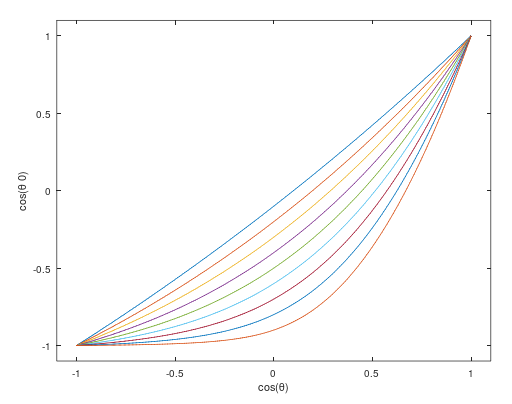
\includegraphics[width=10cm]{chapter_04_paragraph_16_fig_14a}
		\caption{\'Equation (\ref{EQ:16_6}) dans le cas $v_{0} > V$ pour $\dfrac{V}{v_{0}}$ compris entre 0.1 et 0.9 avec un pas de 0.1 et pour $0 < \theta < \pi$}\label{FIG:4_14A}
	\end{center}
\end{figure}

Dans le cas o\`u $v_{0} > V$, le vecteur $\vec{v}$ ne croise le cercle de rayon $v_{0}$ qu'en un unique point et comme il est n\'ecessaire de choisir $\theta_{0} = 0$ quand $\theta = 0$, la solution (\ref{EQ:16_6}) se r\'eduit \`a $\cos\theta_{0} = -\dfrac{V}{v_{0}}\sin^{2}\theta + \cos\theta\sqrt{1 - \dfrac{V^{2}}{v_{0}^{2}}\sin^{2}\theta}$. Ce cas est repr\'esent\'e sur la figure (\ref{FIG:4_14A}) Dans le cas o\`u $v_{0} < V$, le vecteur $\vec{v}$ croise le m\^eme cercle en deux points, B et C sur la figure correspondante (\ref{FIG:4_14}) tel qu'il existe alors deux valeurs de $\theta_{0}$ pour chaque valeur de $\theta$. Ce cas est illustr\'e sur la figure (\ref{FIG:4_14B}).

\begin{figure}[htb!]
	\begin{center}
		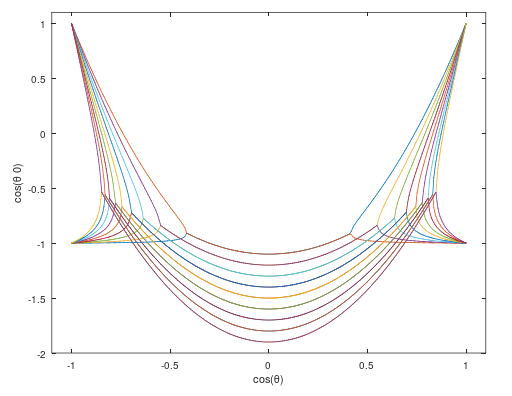
\includegraphics[width=10cm]{chapter_04_paragraph_16_fig_14b}
		\caption{Deux solutions de l'\'equation (\ref{EQ:16_6}) dans le cas $v_{0} < V$ pour $\dfrac{V}{v_{0}}$ compris entre 1.1 et 1.9 avec un pas de 0.1 et pour $0 < \theta < \pi$}\label{FIG:4_14B}
	\end{center}
\end{figure}

Dans la plupart des applications physiques, ce sont de nombreuses particules qui se d\'esint\`egrent et il faut alors raisonner en termes de distribution, en \'energie, en impulsion, en directions, etc. Prenons d\'esormais l'hypoth\`ese de particules initiales orient\'ees de mani\`ere chaotique, i.e. en moyenne de fa\c{c}on isotrope. Dans le r\'ef\'erentiel <<~c~>>, l'isotropie est conserv\'ee apr\`es les d\'esint\'egrations et les particules r\'esultantes de m\^eme esp\`ece ont alors la m\^eme \'energie et la r\'epartition des trajectoires est isotrope. L'orientation chaotique peut se traduire comme la quantit\'e de particules traversant un angle solide\footnote{Par d\'efinition, un \'el\'ement d'angle solide est d\'efini par $\mathrm{d}^{2}\Omega = \dfrac{\vec{r}\cdot\vec{n}}{r^{3}}\mathrm{d}^{2}S$ avec $\vec{r}$ le vecteur rayon et $\vec{n}$ le vecteur normale de l'\'el\'ement de surface $\mathrm{d}^{2}S$. Dans le cadre d'une sph\`ere, nous avons $\mathrm{d}^{2}S = r\mathrm{d}\theta r\sin\theta\mathrm{d}\varphi$ et par cons\'equent $\mathrm{d}^{2}\Omega = \sin\theta\mathrm{d}\theta\mathrm{d}\varphi$ ou encore $\mathrm{d}\Omega = 2\pi\sin\theta\mathrm{d}\theta$.} $\mathrm{d}\omega_{0}$ qui est proportionnelle \`a la grandeur de cet \'el\'ement soit $\frac{\mathrm{d}\omega_{0}}{4\pi}$. Dans le cadre d'une sph\`ere, $\mathrm{d}\omega_{0} = 2\pi\sin\theta_{0}\mathrm{d}\theta_{0}$, donc :
\be
	\dfrac{\mathrm{d}\omega_{0}}{4\pi} = \dfrac{1}{2}\sin\theta_{0}\mathrm{d}\theta_{0} \label{EQ:16_7}
\ee
Pour obtenir la r\'epartition dans le r\'ef\'erentiel <<~l~>>, partons du calcul de l'\'energie cin\'etique et de sa distribution. Nous savons que :
\bea
	\vec{v} & = & \vec{V} + \vec{v}_{0} \nonumber \\
	\Leftrightarrow v^{2} & = & v_{0}^{2} + V^{2} + 2v_{0}V\cos\theta_{0} \nonumber \\
	\Leftrightarrow \cos\theta_{0} & = & \dfrac{v^{2} - v_{0}^{2} - V^{2}}{2v_{0}V}
\eea
Or par rapport \`a $\theta_{0}$, les quantit\'es $\lVert\vec{v}_{0}\rVert$ et $\lVert\vec{V}\rVert$ sont constantes au contraire de $\lVert\vec{v}\rVert$ aussi, nous pouvons en conclure que :
\be
	\mathrm{d}\cos\theta_{0} = -\sin\theta_{0}\mathrm{d}\theta_{0} = \dfrac{\mathrm{d}(v^{2})}{2v_{0}V}
\ee
Or l'\'energie cin\'etique d'une particule r\'esultante de masse $m$ s\'ecrit $T = \frac{1}{2}mv^{2} \Leftrightarrow \mathrm{d}T = \frac{1}{2}m\mathrm{d}(v^{2})$. Donc en reprenant l'\'equation (\ref{EQ:16_7}) :
\bea
	\dfrac{\mathrm{d}\omega_{0}}{4\pi} & = & \dfrac{1}{2}\pi\sin\theta_{0}\mathrm{d}\theta_{0} = -\dfrac{\mathrm{d}(v^{2})}{4v_{0}V} \nonumber \\
	\Leftrightarrow \dfrac{\mathrm{d}\omega_{0}}{4\pi} & = & -\dfrac{\mathrm{d}(T)}{4mv_{0}V} \label{EQ:16_8}
\eea
En reprenant $v^{2} = v_{0}^{2} + V^{2} + 2v_{0}V\cos\theta_{0}$, nous en d\'eduisons que :
\begin{itemize}
	\item l'\'energie cin\'etique maximale est obtenue pour $\theta_{0} = 0$ et $T_{max} = \frac{m}{2}(v_{0} + V)^{2}$
	\item l'\'energie cin\'etique minimale est obtenue pour $\theta_{0} = \pi$ et $T_{max} = \frac{m}{2}(v_{0} - V)^{2}$
\end{itemize}
et dans cet intervalle, l'\'energie cin\'etique se distribue suivant la relation (\ref{EQ:16_8}).

Si la d\'esint\'egration donne plus de deux composantes, cela complexifie l'\'etude et en particulier, l'\'energie des composantes est loin d'\^etre unique dans le r\'ef\'erentiel <<~c~>>. Toutefois il existe une valeur maximale de l'\'energie cin\'etique pour chaque particule r\'esultante. Parmi l'ensemble des particules r\'esultants, consid\'erons-en une de masse $m_{1}$ et en posant $E_{int}'$, l'\'energie <<~interne~>> de l'ensemble des particules restantes moins $m_{1}$. Puisque cette situation permet de revenir \`a un probl\`eme \`a deux corps, la formule (\ref{EQ:16_1}) permet d'\'ecrire :
\be
	E_{int} = E_{int}' + T' + T_{10} + E_{1int}
\ee
avec $T'$ l'\'energie cin\'etique de l'ensemble des particules restantes moins $m_{1}$, $T_{10}$ l'\'energie cin\'etique de $m_{1}$ et $E_{1int}$ son \'energie interne. Les \'energies cin\'etiques peuvent s'\'ecrire avec $M$ la masse de la particule initiale :
\be
	T' = \dfrac{p_{0}^{2}}{2(M - m_{1})}\text{ et }T_{10} = \dfrac{p_{0}^{2}}{2m_{1}}
\ee
donc :
\bea
	E_{int} - E_{int}' - E_{1int} & = & \dfrac{M}{M - m_{1}}\dfrac{p_{0}^{2}}{2m_{1}} \nonumber \\
	\Leftrightarrow T_{10} & = & \dfrac{M - m_{1}}{M}(E_{int} - E_{int}' - E_{1int})
\eea
Aussi $T_{10}$ est maximale si et seulement si $E_{int}'$ est minimale. Ceci intervient lorsque toutes les particules r\'esultantes, sauf $m_{1}$, ont la m\^eme vitesse, i.e. une agitation du syst\`eme minimale et $E_{int}'$ devient simplement la somme des \'energies internes de cet ensemble de particules. Dans ce cas pr\'ecis, la quantit\'e $E_{int} - E_{int}' - E_{1int}$ repr\'esente $\epsilon$, l'\'energie de d\'esint\'egration d\'efinie dans l'\'equation (\ref{EQ:16_2}). Nous en concluons :
\be
	T_{10max} = \dfrac{M - m_{1}}{M}\epsilon \label{EQ:16_9}
\ee

\section{Chocs \'elastiques des particules}

Le choc entre deux particules est dit \'elastique lorsqu'il n'y a pas de modifications de leur \'etat interne. Lors de l'application de la loi de conservation de l'\'energie, il n'est donc pas n\'ecessaire de prendre en compte les \'energies internes respectives. Dans le r\'ef\'erentiel du centre d'inertie <<~c~>>, ce dernier est de facto au repos. Avant le choc, par application de la conservation de l'impulsion, nous avons dans <<~c~>> : $m_{1}\vec{v}_{10} + m_{2}\vec{v}_{20} = \vec{0}$. Dans <<~l~>>, la position du centre d'inertie s'\'ecrit :
\be
	\vec{R} = \dfrac{m_{1}\vec{r}_{1} + m_{2}\vec{r}_{2}}{m_{1} + m_{2}}
\ee
et la loi de composition des vitesses am\`ene \`a \'ecrire :
\be
	\begin{cases}
		\vec{v}_{1} = \vec{v}_{10} + \frac{\mathrm{d}\vec{R}}{\mathrm{dt}} \\
		\vec{v}_{2} = \vec{v}_{20} + \frac{\mathrm{d}\vec{R}}{\mathrm{dt}}
	\end{cases}
\ee
donc en soustrayant les deux relations et en d\'efinissant\footnote{Voir une \'equivalence avec les relations (\ref{EQ:13_2})} $\vec{v} = \vec{v}_{1} - \vec{v}_{2}$ :
\be
	\vec{v} = \vec{v}_{10} - \vec{v}_{20}
\ee
En reprenant la conservation de l'impulsion dans <<~c~>>, nous avons alors :
\be
	\begin{cases}
		\vec{v} = \vec{v}_{10} + \frac{m_{1}}{m_{2}}\vec{v}_{10} \Leftrightarrow \vec{v}_{10} = \frac{m_{2}}{m_{1} + m_{2}}\vec{v} \\
		\vec{v} = -\vec{v}_{20} - \frac{m_{2}}{m_{1}}\vec{v}_{20} \Leftrightarrow \vec{v}_{20} = -\frac{m_{1}}{m_{1} + m_{2}}\vec{v}
	\end{cases}
\ee

Comme le choc est \'elastique, dans <<~c~>>, la conservation de l'impulsion après le choc donne $m_{1}\vec{v'}_{10} + m_{2}\vec{v'}_{20} = \vec{0}$ et comme avant le choc, nous avons $m_{1}\vec{v}_{10} + m_{2}\vec{v}_{20} = \vec{0}$, nous pouvons en conclure que c'est vrai si $m_{1}(\vec{v'}_{10} + \vec{v}_{10}) + m_{2}(\vec{v'}_{20} + \vec{v}_{20}) = \vec{0}$, soit $\vec{v'}_{10} = -\vec{v}_{10}$ et $\vec{v'}_{20} = -\vec{v}_{20}$. De m\^eme, la conservation de l'\'energie avant et apr\`es le choc, et qui ne concerne que les \'energies cin\'etiques, implique que l'\'energie de chacune des deux particules est conserv\'ees car $v'_{10} = v_{10}$ et $v'_{20} = v_{20}$.
Par cons\'equent, dans <<~c~>>, l'unique diff\'erence entre avant et apr\`es le choc se situe dans l'inversion de la direction de la vitesse de chacune des deux particules.

D\'efinissons le vecteur unitaire $\vec{n}_{0}$ dans la direction de la vitesse apr\`es le choc de la particule de masse $m_{1}$. Alors $\vec{v'}_{10} = v'_{10}\vec{n}_{0} = v_{10}\vec{n}_{0}$. Le vecteur $\vec{n}_{0}$ absorbe l'inversion de direction apr\`es le choc et permet de reprendre les relations ci-dessous pour en conclure :
\be
	\begin{cases}
		\vec{v'}_{10} = \frac{m_{2}}{m_{1} + m_{2}}v\vec{n}_{0} \\
		\vec{v'}_{20} = -\frac{m_{1}}{m_{1} + m_{2}}v\vec{n}_{0} \label{EQ:17_1}
	\end{cases}
\ee
Le passage de <<~c~>> \`a <<~l~>> via la loi de composition des vitesses et l'expression de la vitesse du centre d'inertie dans <<~l~>> permet d'\'ecrire :
\be
	\begin{cases}
		\vec{v'}_{1} = \vec{v'}_{10} + \frac{\mathrm{d}\vec{R'}}{\mathrm{dt}} \\
		\vec{v'}_{2} = \vec{v'}_{20} + \frac{\mathrm{d}\vec{R'}}{\mathrm{dt}}
	\end{cases}
\ee
avec :
\be
	\dfrac{\mathrm{d}\vec{R'}}{\mathrm{dt}} = \dfrac{m_{1}\vec{v'}_{1} + m_{2}\vec{v'}_{2}}{m_{1} + m_{2}} = \dfrac{m_{1}\vec{v}_{1} + m_{2}\vec{v}_{2}}{m_{1} + m_{2}}
\ee
par l'additivit\'e des int\'egrales du mouvement, voir le paragraphe (\ref{PAR:6}) qui implique que les lois de conservation ne d\'ependent pas des interactions en jeu, en particulier pour celle de l'impulsion ici. Par cons\'equent, en reportant les \'equations (\ref{EQ:17_1}) :
\be
	\begin{cases}
		\vec{v'}_{1} = \frac{m_{2}}{m_{1} + m_{2}}v\vec{n}_{0} + \frac{m_{1}\vec{v}_{1} + m_{2}\vec{v}_{2}}{m_{1} + m_{2}} \\
		\vec{v'}_{2} = -\frac{m_{1}}{m_{1} + m_{2}}v\vec{n}_{0} + \frac{m_{1}\vec{v}_{1} + m_{2}\vec{v}_{2}}{m_{1} + m_{2}} \label{EQ:17_2}
	\end{cases}
\ee
o\`u seul le vecteur $\vec{n}_{0}$ est une cons\'equence de la loi d'interaction entre les particules. En multipliant les relations (\ref{EQ:17_2}) par la masse respective des particules, nous arrivons \`a exprimer leur impulsion apr\`es le choc en fonction de celle avant le choc, le tout dans le r\'ef\'erentiel <<~l~>> :
\be
	\begin{cases}
		\vec{p'}_{1} = mv\vec{n}_{0} + \frac{m_{1}}{m_{1} + m_{2}}(\vec{p}_{1} + \vec{p}_{2}) \\
		\vec{p'}_{2} = -mv\vec{n}_{0} + \frac{m_{2}}{m_{1} + m_{2}}(\vec{p}_{1} + \vec{p}_{2}) \label{EQ:17_3}
	\end{cases}
\ee
avec $m$ la masse r\'eduite du syt\`eme d\'efinie telle que $m = \frac{m_{1}m_{2}}{m_{1} + m_{2}}$.

\begin{figure}[htb!]
	\begin{center}
		\begin{picture}(300,300)(0,0)
			%circle
			\linethickness{0.05mm}
			\put(150,150){\circle{200}}
			%vectors circle
			\linethickness{0.5mm}
			\put(60,150){\vector(1,0){90}}
			\put(150,150){\vector(1,0){50}}
			\put(60,150){\vector(7,6){115}}\put(90,190){$\vec{p'}_{1}$}
			\put(150,150){\vector(1,5){20}}\put(160,185){$\vec{n}_{0}$}
			\put(170,246){\vector(3,-10){29}}\put(195,190){$\vec{p'}_{2}$}
			%points circle
			\put(146,138){$O$}
			\put(51,148){$A$}
			\put(202,146){$B$}
			\put(175,250){$C$}
		\end{picture}
		\caption{Repr\'esentation g\'eom\'etrique d'un choc entre deux particules}\label{FIG:4_15}
	\end{center}
\end{figure}

Sur la figure (\ref{FIG:4_15}) est trac\'e le cercle de rayon $mv$. Les vecteurs $\vec{AC}$ et $\vec{CB}$ donnent respectivement $\vec{p'}_{1}$ et $\vec{p'}_{2}$ en accord avec les relations (\ref{EQ:17_3}). Les impulsions initiales $\vec{p}_{1}$ et $\vec{p}_{2}$ impliquent que les points $A$ et $B$ ne changent pas de position, aussi seul le point $C$ peut avoir une position quelconque sur le cercle de rayon $mv$. Par construction g\'eom\'etrique, les relations (\ref{EQ:17_3}) donnent :
\be
	\begin{cases}
		\vec{AO} = \frac{m_{1}}{m_{1} + m_{2}}(\vec{p}_{1} + \vec{p}_{2}) \\
		\vec{OB} = \frac{m_{2}}{m_{1} + m_{2}}(\vec{p}_{1} + \vec{p}_{2})
	\end{cases}
\ee

\subsection{Cas de la particule $m_{2}$ au repos avant le choc}

\begin{figure}[htb!]
	\begin{center}
		\begin{picture}(500,300)(0,0)
			%circles
			\linethickness{0.05mm}
			\put(100,150){\circle{200}}\put(90,25){$m_{1} < m_{2}$}
			\put(400,150){\circle{200}}\put(390,25){$m_{1} > m_{2}$}
			%vectors circle #1
			\linethickness{0.5mm}
			\put(40,150){\vector(1,0){160}}
			\put(40,150){\vector(9,5){130}}\put(90,190){$\vec{p'}_{1}$}
			\put(169,221){\vector(3,-7){32}}\put(165,180){$\vec{p'}_{2}$}
			%angles circle #1
			\linethickness{0.05mm}
			\multiput(100,150)(10,10){7}{\line(1,1){8}}
			\qbezier(55,150)(55,155)(50,155)\put(60,153){$\theta_{1}$}
			\qbezier(110,150)(110,155)(105,155)\put(114,154){$\xi$}
			\qbezier(180,150)(188,165)(194,165)\put(170,155){$\theta_{2}$}
			%points circle #1
			\put(95,135){$O$}
			\put(30,147){$A$}
			\put(202,147){$B$}
			\put(175,220){$C$}
			%vectors circle #2
			\linethickness{0.5mm}
			\put(250,150){\vector(1,0){250}}
			\put(250,150){\vector(10,3){220}}\put(390,200){$\vec{p'}_{1}$}
			\put(469,221){\vector(3,-7){32}}\put(465,180){$\vec{p'}_{2}$}
			%\theta_{max} case
			\linethickness{0.05mm}
			\put(250,150){\line(10,9){90}}
			\put(400,150){\line(-11,15){60}}
			%angles circle #2
			\linethickness{0.05mm}
			\multiput(400,150)(10,10){7}{\line(1,1){8}}
			\qbezier(280,150)(280,158)(275,158)\put(287,152){$\theta_{1}$}
			\qbezier(410,150)(410,155)(405,155)\put(412,153){$\xi$}
			\qbezier(480,150)(488,165)(494,165)\put(470,155){$\theta_{2}$}
			\qbezier(320,150)(320,190)(294,190)\put(315,182){$\theta_{max}$}
			%points circle #2
			\put(395,135){$O$}
			\put(240,147){$A$}
			\put(502,147){$B$}
			\put(475,220){$C$}
		\end{picture}
		\caption{Repr\'esentation g\'eom\'etrique de d\'esint\'egrations dans le cas $\vec{v}_{2} = \vec{0}$}\label{FIG:4_16}
	\end{center}
\end{figure}

Si la particule de masse $m_{2}$ est au repos avant le choc, cela se traduit par $v_{2} = \vec{0} = p_{2}$. Nous avons aussi :
\be
	\vec{OB} = \dfrac{m_{2}}{m_{1} + m_{2}}(\vec{p}_{1} + \vec{p}_{2}) = \frac{m_{1}m_{2}}{m_{1} + m_{2}}\vec{v}_{1} = m\vec{v}_{1} = m\vec{v}
\ee
car par d\'efinition, $\vec{v} = \vec{v}_{1} - \vec{v}_{2}$ et donc \'egal \`a $\vec{v}_{1}$ dans le cas qui nous occupe. Donc le point $B$ se trouve positionner sur le cercle de rayon $mv$. De plus :
\be
	\vec{AB} = \vec{AO} + \vec{OB} = \frac{m_{1}}{m_{1} + m_{2}}\vec{p}_{1} + \dfrac{m_{2}}{m_{1} + m_{2}}\vec{p}_{1} = \vec{p}_{1}
\ee
Le vecteur $\vec{AB}$ repr\'esente donc l'impulsion de d\'epart de la particule de masse $m_{1}$.

Les points $A$, $O$ et $B$ se situant sur la m\^eme droite, nous pouvons en d\'eduire :
\be
	AO = AB - OB = m_{1}v_{1} - \dfrac{m_{1}m_{2}}{m_{1} + m_{2}}v_{1} = \dfrac{m_{1}^{2}}{m_{1} + m_{2}}v_{1} = \dfrac{m_{1}}{m_{2}}OB
\ee
Par cons\'equent :
\begin{itemize}
	\item si $m_{1} < m_{2}$ alors le point $A$ se situe \`a l'int\'erieur du cercle
	\item si $m_{1} = m_{2}$ alors le point $A$ se situe sur le cercle
	\item si $m_{1} > m_{2}$ alors le point $A$ se situe \`a l'ext\'erieur du cercle
\end{itemize}
Ces cas sont repr\'esent\'es sur la figure (\ref{FIG:4_16}). Sur celle-ci, les angles $\theta_{1}$ et $\theta_{2}$ sont les angles de d\'eviation dans <<~l~>> par rapport \`a la direction du choc, d\'efinie par $\vec{p}_{1}$ et $\xi$ est l'angle de d\'eviation de la particule de masse $m_{1}$ dans <<~c~>>. Les angles $\theta_{1}$ et $\theta_{2}$ peuvent \^etre calcul\'es ainsi :
\be
	\begin{cases}
		\tan\theta_{1} = \dfrac{mv\sin\xi}{AO + mv\cos\xi} = \dfrac{\dfrac{m_{1}m_{2}}{m_{1} + m_{2}}v\sin\xi}{\dfrac{m_{1}^{2}}{m_{1} + m_{2}}v + \dfrac{m_{1}m_{2}}{m_{1} + m_{2}}v\cos\xi} = \dfrac{m_{2}\sin\xi}{m_{1} + m_{2}\cos\xi} \\
		\\
		\pi = \dfrac{\pi}{2} + \dfrac{\xi}{2} + \theta_{2} \Leftrightarrow \theta_{2} = \dfrac{\pi - \xi}{2} \label{EQ:17_4}
	\end{cases}
\ee

D\'eterminons ensuite la valeur de la vitesse apr\`es le choc pour les deux particules dans <<~l~>>. Nous avons d\'ej\`a vu que $\vec{v'}_{1} = \vec{v'}_{10} + \vec{\dot{R'}}$ sachant que $\vec{\dot{R'}} = \vec{\dot{R}}$, aussi :
\be
	{v'}_{1}^{\,2} = {v'}_{10}^{\,2} + {\lVert \vec{\dot{R}} \rVert}^{2} + 2v'_{10}\lVert \vec{\dot{R}} \rVert\cos\theta_{10}
\ee
or $\theta_{10} = \xi$ par d\'efinition, donc :
\be
	{v'}_{1}^{\,2} = \dfrac{m_{2}^{2}}{(m_{1} + m_{2})^{2}}v^{2} + \dfrac{m_{1}^{2}}{(m_{1} + m_{2})^{2}}v_{1}^{2} + 2\dfrac{m_{1}m_{2}}{(m_{1} + m_{2})^{2}}vv_{1}\cos\xi
\ee
et comme $v_{1} = v$, nous avons :
\be
	v'_{1} = \dfrac{\sqrt{m_{1}^{2} + m_{2}^{2} + 2m_{1}m_{2}\cos\xi}}{m_{1} + m_{2}}v \label{EQ:17_5A}
\ee
De mani\`ere similaire pour $v'_{2}$, nous avons $\vec{v'}_{1} = \vec{v'}_{10} + \vec{\dot{R}}$, soit :
\bea
	{v'}_{2}^{\,2} & = & {v'}_{20}^{\,2} + {\lVert \vec{\dot{R}} \rVert}^{2} + 2v'_{20}\lVert \vec{\dot{R}} \rVert\cos(\langle \vec{v'}_{20},\vec{\dot{R}} \rangle) \nonumber \\
	& = & \dfrac{m_{1}^{2}}{(m_{1} + m_{2})^{2}}v^{2} + \dfrac{m_{1}^{2}}{(m_{1} + m_{2})^{2}}v_{1}^{2} + 2\dfrac{m_{1}^{2}}{(m_{1} + m_{2})^{2}}vv_{1}\cos\theta_{20}
\eea
et comme $v_{1} = v$ et $\theta_{20} = \pi - \xi$ :
\bea
	{v'}_{2}^{\,2} & = &  2\dfrac{m_{1}^{2}}{(m_{1} + m_{2})^{2}}v^{2} - 2\dfrac{m_{1}^{2}}{(m_{1} + m_{2})^{2}}v^{2}\cos\xi \nonumber \\
	& = & 2\dfrac{m_{1}^{2}}{(m_{1} + m_{2})^{2}}v^{2}(1 - \cos\xi) = 2\dfrac{m_{1}^{2}}{(m_{1} + m_{2})^{2}}v^{2}\left(1 - 1 + 2\sin^{2}\left(\dfrac{\xi}{2}\right)\right) \nonumber \\
	& = & 4\dfrac{m_{1}^{2}}{(m_{1} + m_{2})^{2}}v^{2}\sin^{2}\left(\dfrac{\xi}{2}\right)
\eea
car :
\be
	\cos\xi = \cos\left(\dfrac{\xi}{2} + \dfrac{\xi}{2}\right) = \cos^{2}\left(\dfrac{\xi}{2}\right) - \sin^{2}\left(\dfrac{\xi}{2}\right) = 1 - 2\sin^{2}\left(\dfrac{\xi}{2}\right)
\ee
Nous arrivons donc \`a :
\be
	v'_{2} = \dfrac{m_{1}}{m_{1} + m_{2}}v\sin\left(\dfrac{\xi}{2}\right) \label{EQ:17_5B}
\ee

Les deux particules \`a l'issue du choc s'\'ecartent l'une de l'autre avec un angle $\theta_{1} + \theta_{2}$. Sur la figure (\ref{FIG:4_16}), si $m_{1} < m_{2}$ alors l'angle $\langle \vec{CA},\vec{CB} \rangle < \frac{\pi}{2}$ donc $\theta_{1} + \theta_{2} = \pi - \langle \vec{CA},\vec{CB} \rangle > \frac{\pi}{2}$. Et le point $C$ peut tout \`a fait prendre n'importe quelle place sur le cercle de rayon $mv$, i.e. la premi\`ere particule de masse $m_{1}$ peut donc s'\'echapper suivant une direction quelconque.

Dans le cas contraire o\`u $m_{1} > m_{2}$ alors $\theta_{1} + \theta_{2} < \frac{\pi}{2}$. Dans ce cas, le point $C$ donne une valeur maximale \`a l'angle $\theta_{1}$, \`a l'emplacement exact o\`u $CA \perp CO$, soit :
\be
	\sin\theta_{1max} = \dfrac{CO}{AO} = \dfrac{OB}{AO} = \dfrac{OB}{\frac{m_{1}}{m_{2}}OB} = \dfrac{m_{2}}{m_{1}} \label{EQ:17_8}
\ee

\subsection{Choc de front}

Examinons le cas o\`u les deux particules se meuvent apr\`es le choc sur une m\^eme droite, i.e. $\xi = \pi$, en gardant l'hypoth\`ese $\vec{v}_{2} = \vec{0}$. En reprenant la figure (\ref{FIG:4_15}), nous pouvons positionner les points tels que :
\begin{itemize}
	\item si $m_{1} < m_{2}$ : A, O, B puis C impliquant que dans ce cas, les vecteurs $\vec{p'}_{1}$ et $\vec{p'}_{2}$ sont de sens oppos\'e
	\item si $m_{1} > m_{2}$ : A, C, O et B impliquant que dans ce cas, les vecteurs $\vec{p'}_{1}$ et $\vec{p'}_{2}$ sont de m\^eme sens
\end{itemize}
En utilisant les relations (\ref{EQ:17_5A}) et (\ref{EQ:17_5B}) avec $\xi = \pi$, nous obtenons :
\bea
	v'_{1} & = & \dfrac{\sqrt{m_{1}^{2} + m_{2}^{2} - 2m_{1}m_{2}}}{m_{1} + m_{2}}v = \dfrac{m_{1} - m_{2}}{m_{1} + m_{2}}v \nonumber \\
	v'_{2} & = & \dfrac{m_{1}}{m_{1} + m_{2}}v \label{EQ:17_6}
\eea
En calculant $v'_{2} - v'_{1}$ :
\be
	v'_{2} - v'_{1} = \dfrac{2m_{1} - (m_{1} - m_{2})}{m_{1} + m_{2}}v = \dfrac{m_{1} + m_{2}}{m_{1} + m_{2}}v = v > 0
\ee
nous pouvons en d\'eduire que $v'_{2} > v'_{1}$ donc l'\'energie maximale de la particule initialement au repos, et de masse $m_{2}$ est, apr\`es le choc :
\be
	E'_{2max} = \dfrac{m_{2}}{2}{v'}_{2}^{2} = 2\dfrac{m_{1}^{2}m_{2}}{(m_{1} + m_{2})^{2}}v^{2} = 2\dfrac{m_{2}m_{1}^{2}v_{1}^{2}}{(m_{1} + m_{2})^{2}} = 4\dfrac{m_{1}m_{2}}{(m_{1} + m_{2})^{2}}E_{1} \label{EQ:17_7}
\ee
avec $E_{1} = \dfrac{1}{2}m_{1}v_{1}^{2}$ qui est l'\'energie initiale de la particule incident, de masse $m_{1}$.

\subsection{Cas d'un choc entre deux particules de même masse dont l'une au repos avant le choc}

\begin{figure}[htb!]
	\begin{center}
		\begin{picture}(300,300)(0,0)
			%circles
			\linethickness{0.05mm}
			\put(150,150){\circle{200}}
			%vectors circle #1
			\linethickness{0.5mm}
			\put(50,150){\vector(1,0){200}}
			\put(50,150){\vector(9,4){170}}\put(140,200){$\vec{p'}_{1}$}
			\put(219,221){\vector(3,-7){32}}\put(215,180){$\vec{p'}_{2}$}
			%angles circle #1
			\linethickness{0.05mm}
			\multiput(150,150)(10,10){7}{\line(1,1){8}}
			\qbezier(65,150)(65,155)(60,155)\put(75,153){$\theta_{1}$}
			\qbezier(160,150)(160,155)(155,155)\put(164,154){$\xi$}
			\qbezier(230,150)(238,165)(244,165)\put(220,155){$\theta_{2}$}
			%points circle #1
			\put(145,135){$O$}
			\put(40,147){$A$}
			\put(252,147){$B$}
			\put(225,220){$C$}
		\end{picture}
		\caption{Repr\'esentation g\'eom\'etrique de d\'esint\'egrations dans le cas $\vec{v}_{2} = \vec{0}$ et $m_{1} = m_{2}$}\label{FIG:4_17}
	\end{center}
\end{figure}

Dans ce cas et comme d\'ej\`a montr\'e pr\'ec\'edemment, les points $A$ et $B$ se trouvent sur le cercle comme illustr\'e sur la figure (\ref{FIG:4_17}) et de facto, le triangle form\'e par les points $A$, $B$ et $C$ est rectangle. Par cons\'equent, nous avons :
\be
	\theta_{1} = \dfrac{\xi}{2}\text{ et }\theta_{2} = \dfrac{\pi - \xi}{2} \label{EQ:17_9}
\ee
et remarquons que $\theta_{2} - \theta_{1} = \frac{\pi}{2}$, i.e. que les deux particules s'éloignent l'une de l'autre sous un angle droit. Enfin, dans ce triangle rectangle, nous pouvons noter :
\be
	\begin{cases}
		p'_{1} = mv'_{1} = mv\cos\frac{\xi}{2} \Leftrightarrow v'_{1} = v\cos\frac{\xi}{2} \\
		p'_{2} = mv'_{2} = mv\sin\frac{\xi}{2} \Leftrightarrow v'_{2} = v\sin\frac{\xi}{2} \label{EQ:17_10}
	\end{cases}
\ee

\section{Diffusion des particules}

Dans le paragraphe pr\'ec\'edent, nous avons \'etudi\'e les param\`etres de la trajectoire des particules apr\`es le choc \`a partir des \'el\'ements avant le choc. Mais pour d\'eterminer pleinement le r\'esultat du choc, il faut tenir compte de la loi d'interaction entre les particules. Consid\'erons d'abord la d\'eviation d'une particule de masse $m$ dans un champ d'\'energie potentielle $U(r)$ o\`u` le centre de force\footnote{Le centre de force est le point tel que $r = 0$  dans le champ de force, i.e. le champ d'\'energie potentielle} est immobile, i.e. plac\'e \`a la position du centre d'inertie du syst\`eme de particules.

Le point de rebroussement d\'efini par $\dot{r} = 0$ entre les \'equations (\ref{EQ:14_8}) et (\ref{EQ:14_10}) implique que la trajectoire est sym\'etrique par rapport à ce point, qui, de facto correspond au p\'erih\'elie de la trajectoire, voir la figure (\ref{FIG:4_18}). Sur celle-ci, $\xi$ correspond \`a l'angle de d\'eviation par rapport \`a la direction initiale de la particule. $\varphi_{0}$ est l'angle de d\'eviation lorsque la particule passe au plus pr\`es du centre du champ de force, soit le p\'erih\'elie. Par construction, nous avons :
\be
	\xi = \lvert \pi - 2\varphi_{0} \rvert \label{EQ:18_1}
\ee
et par application de l'\'equation (\ref{EQ:14_7}) :
\be
	\varphi_{0} = \bigintsss{r_{min}}^{+\infty}{\dfrac{\frac{M}{r^{2}}\mathrm{d}r}{\sqrt{2m(E - U(r)) - \frac{M^{2}}{r^{2}}}}} \label{EQ:18_2}
\ee
Dans le cadre d'un mouvement infini, il est commode d'\'ecrire l'\'energie $E$ et le moment cin\'etique $M$ en fonction de $v_{\infty}$, la vitesse de la particule incidente pour $r\leftarrow\infty$, et $\rho$, la \emph{distance de vis\'ee}, i.e., la distance minimale par rapport au centre de force s'il n'y avait pas de champ de force. Par conservation de l'\'energie, et parce que $U(\infty) = 0$, et du moment cin\'etique et en accord avec les d\'efinitinos pr\'ec\'edentes, la particule incidente poss\`ede les caract\'eristiques du mouvement suivantes :
\be
	E = \dfrac{mv_{\infty}^{2}}{2}\text{ et } M = m\rho v_{\infty} \label{EQ:18_3}
\ee
L'\'equation (\ref{EQ:18_2}) devient alors dans ce contexte :
\be
	\varphi_{0} = \bigintsss_{r_{min}}^{+\infty}{\dfrac{\frac{m\rho v_{\infty}}{r^{2}}\mathrm{d}r}{\sqrt{2m\left(\dfrac{mv_{\infty}^{2}}{2} - U(r)\right) - \dfrac{m^{2}\rho^{2}v_{\infty}^{2}}{r^{2}}}}} = \bigintsss_{r_{min}}^{+\infty}{\dfrac{\frac{\rho}{r^{2}}\mathrm{d}r}{\sqrt{1 - \dfrac{\rho^{2}}{r^{2}} - \dfrac{2U(r)}{mv_{\infty}^{2}}}}} \label{EQ:18_4}
\ee
Avec l'\'equation (\ref{EQ:18_1}), nous avons donc une relation entre $\xi$ et $\rho$.

Dans les applications physiques, nous avons affaire \`a un faisceau de particules semblables arrivant avec la m\^eme vitesse $v_{\infty}$ mais avec des distances de vis\'ee $\rho$ diff\'erentes. Elles sont alors diffus\'ees suivant des angles $\xi$ diff\'erents. Il s'agit du ph\'enom\`ene de \emph{diffusion}.

\begin{figure}[htb!]
	\begin{center}
		\begin{picture}(300,200)(0,0)
			%dashed lines
			\linethickness{0.05mm}
			\multiput(0,0)(10,0){30}{\line(1,0){8}}
			\multiput(0,50)(10,0){30}{\line(1,0){8}}
			\multiput(25,0)(10,10){10}{\line(1,1){8}}
			\multiput(75,50)(-1,10){15}{\line(-1,8){1}}
			%curve
			\qbezier(65,200)(70,70)(300,55)
			%angles
			\qbezier(40,0)(40,10)(35,10)\put(42,5){$\varphi_{0}$}
			\qbezier(65,50)(65,60)(73,60)\put(60,63){$\xi$}
			%vector
			\put(150,30){\vector(0,1){20}}
			\put(150,20){\vector(0,-1){20}}
			\put(148,23){$\rho$}
			%points
			\put(17,3){$O$}
			\put(123,100){$A$}
		\end{picture}
		\caption{D\'eviation d'une particule dans un champ de force}\label{FIG:4_18}
	\end{center}
\end{figure}

Soit $\mathrm{d}N$ le nombre de particules diffus\'ees par unit\'e de temps dans l'angle compris entre $\xi$ et $\xi + \mathrm{d}\xi$. $\mathrm{d}N$ est par d\'efinition proportionnel \`a la densit\'e du faisceau incident. Soit :
\be
	\mathrm{d}\sigma = \dfrac{\mathrm{d}N}{n} \label{EQ:18_5}
\ee
o\`u $n$ est le nombre de particules traversant l'unit\'e de surface d'une section droite du faisceau incident par unit\'e de temps\footnote{Restons dans l'hypoth\`ese d'un faisceau homog\`ene sur toute sa section.}. Alors la quantit\'e $\mathrm{d}\sigma$ a la dimension d'une surface et est appel\'ee la \emph{section efficace du faisceau}. Ce param\`etre est la caract\'eristique la plus importante du processus de diffusion.

Consid\'erons par hypoth\`ese que $\xi$ et $\rho$ sont r\'eciproquement univoque. D\'emontrons que c'est vrai lorsque $\xi$ est une fonction monotone et d\'ecroissante de $\rho$, i.e. $\forall\rho$, $\frac{\mathrm{d}\xi}{\mathrm{d}\rho} < 0$ et $\forall\xi$, $\frac{\mathrm{d}\rho}{\mathrm{d}\xi} < 0$, donc au premier ordre, le d\'eveloppement de Taylor donne :
\be
	\begin{cases}
		\xi(\rho + \delta\rho) = \xi(\rho) + \frac{\mathrm{d}\xi}{\mathrm{d}\rho}\delta\rho \Rightarrow \xi(\rho + \delta\rho) < \xi(\rho) \\
		\rho(\xi + \delta\xi) = \rho(\xi) + \frac{\mathrm{d}\rho}{\mathrm{d}\xi}\delta\xi \Rightarrow \rho(\xi + \delta\xi) < \rho(\xi)
	\end{cases}
\ee
et nous avons donc bien \'etabli cette relation univoque.

Le nombre de particules diffus\'ees entre $\xi$ et $\xi + \mathrm{d}\xi$ par unit\'e de temps est \'egal au nombre de particules issu du cercle de surface $2\pi\rho(\xi + \mathrm{d}\xi)$ diminu\'e par le nombre de particules issu du cercle de surface $2\pi\rho(\xi)$, soit :
\be
	\mathrm{d}N = 2\pi(\rho(\xi + \mathrm{d}\xi) - \rho(\xi))n = 2\pi\mathrm{d}\rho n
\ee
car au premier ordre, nous avons toujours $\rho(\xi + \mathrm{d}\xi) = \rho(\xi) + \mathrm{d}\rho(\xi)$ et la section efficace d\'efinie \`a l'\'equation (\ref{EQ:18_5}) vaut :
\be
	\mathrm{d}\sigma = 2\pi\mathrm{d}\rho \label{EQ:18_6}
\ee
qui peut aussi s'\'ecrire :
\be
	\mathrm{d}\sigma = 2\pi\rho(\xi)\Bigg\lvert \dfrac{\mathrm{d}\rho(\xi)}{\mathrm{d}\xi} \Bigg\rvert \mathrm{d}\xi \label{EQ:18_7}
\ee
Comme la plupart du temps la valeur de $\frac{\mathrm{d}\rho(\xi)}{\mathrm{d}\xi}$ est n\'egative et que la section efficace est une surface, il est n\'ecessaire d'utiliser la valeur absolue. \'Ecrivons d\'esormais la section efficace en fonction de l'angle solide. Ce dernier vaut pour un anneau $\mathrm{d}\omega = 2\pi\sin\xi\mathrm{d}\xi$, voir la relation (\ref{EQ:16_7}), ce qui permet d'\'ecrire :
\be
	\mathrm{d}\sigma = 2\pi\rho(\xi)\lvert \dfrac{\mathrm{d}\rho(\xi)}{\mathrm{d}\xi} \rvert \dfrac{\mathrm{d}\omega}{2\pi\sin\xi} = \dfrac{\rho(\xi)}{\sin\xi}\lvert \dfrac{\mathrm{d}\rho(\xi)}{\mathrm{d}\xi} \rvert \mathrm{d}\omega \label{EQ:18_8}
\ee
Revenons au cas d'un faisceau de particules diffus\'ees par d'autres particules initialement au repos. Dans la relation (\ref{EQ:18_7}), la section efficace $\mathrm{d}\sigma$ est d\'efinie dans le cadre d'un champ de force positionn\'e au centre d'inertie des particules. $\mathrm{d}\sigma$ est donc bien la section efficace dans le r\'ef\'erentiel <<~c~>> et exprim\'ee en fonction de l'angle de d\'eviation $\xi$. Pour l'exprimer dans le cadre du r\'ef\'erentiel du laboratoire <<~l~>>, nous revenons aux relations (\ref{EQ:17_4}). En fonction de $\theta_{1}$, l'angle de d\'eviation dans <<~l~>> pour les particules du faisceau incident, nous avons :
\bea
	\tan\theta_{1} = \dfrac{m_{2}\sin\xi}{m_{1} + m_{2}\cos\xi} & \Leftrightarrow & \dfrac{\sin^{2}\theta_{1}}{\cos^{2}\theta_{1}} = \dfrac{m_{2}^{2}\sin^{2}\xi}{(m_{1} + m_{2}\cos\xi)^{2}} \nonumber \\
	\sin^{2}\theta_{1}(m_{1}^{2} + m_{2}^{2}\cos^{2}\xi + 2m_{1}m_{2}\cos\xi) & = & m_{2}^{2}\cos^{2}\theta_{1} - m_{2}^{2}\cos^{2}\theta_{1}\cos^{2}\xi \nonumber \\
	m_{1}^{2}\sin^{2}\theta_{1} + m_{2}^{2}\sin^{2}\theta_{1}\cos^{2}\xi + 2m_{1}m_{2}\sin^{2}\theta_{1}\cos\xi & = & m_{2}^{2}\cos^{2}\theta_{1} - m_{2}^{2}\cos^{2}\theta_{1}\cos^{2}\xi \nonumber \\
	(\sin^{2}\theta_{1} + \cos^{2}\theta_{1})m_{2}^{2}\cos^{2}\xi + 2m_{1}m_{2}\sin^{2}\theta_{1}\cos\xi & = & m_{2}^{2}\cos^{2}\theta_{1} - m_{1}^{2}\sin^{2}\theta_{1} \nonumber \\
	\cos^{2}\xi + 2\dfrac{m_{1}}{m_{2}}\sin^{2}\theta_{1}\cos\xi + \dfrac{m_{1}^{2}}{m_{2}^{2}}\sin^{2}\theta_{1} - \cos^{2}\theta_{1} & = & 0
\eea
une \'equation du second degr\'e en $\cos\xi$ dont les solutions sont :
\bea
	\cos\xi & = & \dfrac{-2\dfrac{m_{1}}{m_{2}}\sin^{2}\theta_{1} \pm \sqrt{\dfrac{4m_{1}^{2}}{m_{2}^{2}}\sin^{4}\theta_{1} - 4\left(\dfrac{m_{1}^{2}}{m_{2}^{2}}\sin^{2}\theta_{1} - \cos^{2}\theta_{1}\right)}}{2} \nonumber \\
	& = & -\dfrac{m_{1}}{m_{2}}\sin^{2}\theta_{1} \pm \sqrt{\dfrac{m_{1}^{2}}{m_{2}^{2}}\sin^{2}\theta_{1}(\sin^{2}\theta_{1} - 1) + \cos^{2}\theta_{1}} \nonumber \\
	& = & -\dfrac{m_{1}}{m_{2}}\sin^{2}\theta_{1} \pm \cos\theta_{1}\sqrt{1 - \dfrac{m_{1}^{2}}{m_{2}^{2}}\sin^{2}\theta_{1}}\label{EQ:18_9}
\eea
Et en fonction de $\theta_{2}$ l'angle de d\'eviation dans <<~l~>> pour les particules initialement au repos :
\be
	\theta_{2} = \dfrac{\pi - \xi}{2} \Leftrightarrow \xi = \pi - 2\theta_{2}\label{EQ:18_10}
\ee

\section{Formule de Rutherford}

Int\'eressons-nous d\'esormais à la diffusion de particules charg\'ees dans un champ Coulombien, i.e. tel que $U(r) = \alpha / r$ pour $\alpha > 0$. En appliquant la relation (\ref{EQ:18_4}) pour une particule de masse $m$, nous avons pour $\varphi_{0}$, qui est ,pour rappel, l'angle de d\'eviation au plus pr\`es du centre du champ, i.e. pour $r = r_{min}$ :
\be
	\varphi_{0} = \int_{r_{min}}^{+\infty}{\dfrac{\frac{\rho}{r^{2}}\mathrm{d}r}{\sqrt{1 - \dfrac{\rho^{2}}{r^{2}} - \dfrac{2\alpha}{mv_{\infty}^{2}r}}}}
\ee
En posant :
\be
	\begin{cases}
		x = \dfrac{\rho}{r} - \dfrac{\alpha}{mv_{\infty}^{2}\rho} \Leftrightarrow \dfrac{1}{r} = \dfrac{x}{\rho} - \dfrac{\alpha}{mv_{\infty}^{2}\rho^{2}}\\
		\\
		\mathrm{d}x = -\dfrac{\rho\mathrm{d}r}{r^{2}}
	\end{cases}
\ee
nous avons pour $r = r_{min}$, $x = x_{min}$ et pour $r \rightarrow \infty$, $x = \frac{\alpha}{mv_{\infty}^{2}\rho}$ et :
\bea
	\varphi_{0} & = & \int_{x_{min}}^{\frac{\alpha}{mv_{\infty}^{2}\rho}}\dfrac{-\mathrm{d}x}{\sqrt{1 - \rho^{2}\left(\dfrac{x}{\rho} - \dfrac{\alpha}{mv_{\infty}^{2}\rho^{2}}\right)^{2} - \dfrac{2\alpha}{mv_{\infty}^{2}}\left(\dfrac{x}{\rho} - \dfrac{\alpha^{2}}{mv_{\infty}^{2}\rho^{2}}\right)}} \nonumber \\
	& = & \int_{x_{min}}^{\frac{\alpha}{mv_{\infty}^{2}\rho}}\dfrac{-\mathrm{d}x}{\sqrt{1 - \rho^{2}\dfrac{x^{2}}{\rho^{2}} - \dfrac{\rho^{2}\alpha^{2}}{m^{2}v_{\infty}^{2}\rho^{4}} + 2\rho^{2}\dfrac{\alpha x}{mv_{\infty}^{2}\rho^{3}} - \dfrac{2\alpha x}{mv_{\infty}^{2}\rho} + \dfrac{2\alpha^{2}}{m^{2}v_{\infty}^{4}\rho^{2}}}} \nonumber \\
	& = & \int_{x_{min}}^{\frac{\alpha}{mv_{\infty}^{2}\rho}}\dfrac{-\mathrm{d}x}{\sqrt{1 + \dfrac{\alpha^{2}}{m^{2}v_{\infty}^{2}\rho^{2}} - x^{2}}}
\eea
D\'esormais, posons :
\be
	\begin{cases}
		y = \dfrac{x}{\sqrt{1 + \left(\dfrac{\alpha}{mv_{\infty}^{2}\rho}\right)^{2}}} \Leftrightarrow x^{2} = \left(1 + \left(\dfrac{\alpha}{mv_{\infty}^{2}\rho}\right)^{2}\right)y^{2} \\
		\\
		\mathrm{d}x = \sqrt{1 + \left(\dfrac{\alpha}{mv_{\infty}^{2}\rho}\right)^{2}}\mathrm{d}y
	\end{cases}
\ee
et pour $x = x_{min}$, $y = y_{min}$ et pour $x = \frac{\alpha}{mv_{\infty}^{2}\rho}$, $y = Y = \dfrac{\dfrac{\alpha}{mv_{\infty}^{2}\rho}}{\sqrt{1 + \left(\dfrac{\alpha}{mv_{\infty}^{2}\rho}\right)^{2}}}$, cela donne :
\be
	\varphi_{0} = \int_{y_{min}}^{Y}\dfrac{-\sqrt{1 + \left(\dfrac{\alpha}{mv_{\infty}^{2}\rho}\right)^{2}}\mathrm{d}y}{\sqrt{1 + \left(\dfrac{\alpha}{mv_{\infty}^{2}\rho}\right)^{2}}\sqrt{1 - y^{2}}} = \int_{y_{min}}^{Y}\dfrac{-\mathrm{d}y}{\sqrt{1 - y^{2}}}
\ee
En choisissant la valeur de $y_{min}$ telle que $\varphi_{0}(y_{min}) = 0$, nous arrivons \`a :
\be
	\varphi_{0} = \arccos\left(\dfrac{\dfrac{\alpha}{mv_{\infty}^{2}\rho}}{\sqrt{1 + \left(\dfrac{\alpha}{mv_{\infty}^{2}\rho}\right)^{2}}}\right)
\ee
dont plusieurs repr\'esentations sont visibles sur la figure (\ref{FIG:4_19}).

\begin{figure}[htb!]
	\begin{center}
		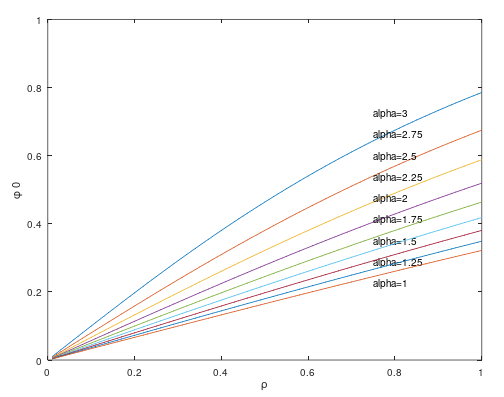
\includegraphics[width=10cm]{chapter_04_paragraph_19}
		\caption{Variation de $\varphi_{0}$ en fonction de la distance de vis\'ee $\rho$ pour plusieurs valeurs de $\alpha$ et pour $mv_{\infty}^{2} = 1$}\label{FIG:4_19}
	\end{center}
\end{figure}
Poursuivons le raisonnement :
\bea
	\cos\varphi_{0}\sqrt{1 + \left(\dfrac{\alpha}{mv_{\infty}^{2}\rho}\right)^{2}} & = & \dfrac{\alpha}{mv_{\infty}^{2}\rho} \Leftrightarrow \cos^{2}\varphi_{0} = \left(\dfrac{\alpha}{mv_{\infty}^{2}\rho}\right)^{2}(1 - \cos^{2}\varphi_{0}) \nonumber \\
	\cos\varphi_{0}\sqrt{1 + \left(\dfrac{\alpha}{mv_{\infty}^{2}\rho}\right)^{2}} & = & \dfrac{\alpha}{mv_{\infty}^{2}\rho} \Leftrightarrow \cos^{2}\varphi_{0} = \left(\dfrac{\alpha}{mv_{\infty}^{2}\rho}\right)^{2}(1 - \cos^{2}\varphi_{0}) \nonumber \\
	\Leftrightarrow \tan^{2}\varphi_{0} & = & \left(\dfrac{mv_{\infty}^{2}\rho}{\alpha}\right)^{2} \Leftrightarrow \rho^{2} = \left(\dfrac{\alpha}{mv_{\infty}^{2}}\right)^{2}\tan^{2}\varphi_{0}
\eea
et en utilisant l'\'equation (\ref{EQ:18_1}) : $\xi = \lvert \pi - 2\varphi_{0} \rvert \Leftrightarrow \varphi_{0} = (\pi - \xi)/2$ et parce que :
\be
	\tan\left(\frac{\pi - \xi}{2}\right) = \dfrac{\sin\left(\frac{\pi - \xi}{2}\right)}{\cos\left(\frac{\pi - \xi}{2}\right)} = \dfrac{\cos\left(\frac{\xi}{2}\right)}{\sin\left(\frac{\xi}{2}\right)} = \dfrac{1}{\tan\left(\frac{\xi}{2}\right)}
\ee
nous avons :
\be
	\rho^{2} = \left(\dfrac{\alpha}{mv_{\infty}^{2}}\right)^{2}\dfrac{1}{\tan\left(\frac{\xi}{2}\right)} \label{EQ:19_1}
\ee
En partant de l'\'equation (\ref{EQ:18_7}), et parce que :
\bea
	\left(\dfrac{1}{\tan\theta}\right)^{'} & = & -\dfrac{\tan'\theta}{\tan^{2}\theta} = -\dfrac{1}{\cos^{2}\theta}\dfrac{\cos^{2}\theta}{\sin^{2}\theta} = -\dfrac{1}{\sin^{2}\theta} \nonumber \\
	\Leftrightarrow \left(\dfrac{1}{\tan(\theta/2)}\right)^{'} & = & -\dfrac{1}{2\sin^{2}(\theta/2)}
\eea
nous pouvons calculer :
\bea
	\mathrm{d}\sigma & = & 2\pi\rho(\xi)\lvert \dfrac{\mathrm{d}\rho(\xi)}{\mathrm{d}\xi} \rvert \mathrm{d}\xi = 2\pi\dfrac{\alpha}{mv_{\infty}^{2}}\dfrac{\cos^{2}(\xi/2)}{\sin^{2}(\xi/2)}\lvert -\dfrac{1}{2\sin^{2}(\theta/2)} \rvert\dfrac{\alpha}{mv_{\infty}^{2}}\mathrm{d}\xi \nonumber \\
	& = & \pi\left(\dfrac{\alpha}{mv_{\infty}^{2}}\right)^{2}\lvert \dfrac{\cos(\xi/2)}{\sin^{3}(\xi/2)} \rvert \mathrm{d}\xi \label{EQ:19_2}
\eea
En remarquant que :
\be
	\mathrm{d}\omega = 2\pi\sin\xi\mathrm{d}\xi = 2\pi\cdot 2\cos(\xi/2)\sin(\xi/2)\mathrm{d}\xi \Leftrightarrow \pi\cos(\xi/2)\mathrm{d}\xi = \dfrac{\mathrm{d}\omega}{4\sin(\xi/2)}
\ee
alors l'\'equation (\ref{EQ:19_2}) devient :
\be
	\mathrm{d}\sigma = \left(\dfrac{\alpha}{mv_{\infty}^{2}}\right)^{2}\dfrac{\mathrm{d}\omega}{4\sin^{4}(\xi/2)} \label{EQ:19_3}
\ee
qui est la \emph{formule de Rutherford} dont nous pouvons remarquer qu'elle ne d\'epend pas du signe de $\alpha$ et que cette formule est donc identique pour un champ coulombien attractif ou r\'epulsif. Elle est ici donn\'ee dans le r\'ef\'erentiel du centre d'inertie au repos puisque nous avons utilis\'e l'\'equation (\ref{EQ:18_2}) pour le calcul de $\varphi_{0}$. Pour passer au r\'ef\'erentiel du laboratoire, il nous faut utiliser les relations (\ref{EQ:17_4}). Dans <<~l~>>, $m$ est la masse r\'eduite et pour les particules initialement au repos, $\xi = \pi - 2\theta_{2} \Leftrightarrow \mathrm{d}\xi = -2\mathrm{\theta_{2}}$. Ainsi, l'\'equation (\ref{EQ:19_2}) devient dans <<~l~>> :
\be
	\mathrm{d}\sigma_{2} = \lvert -2\pi\left(\dfrac{\alpha}{mv_{\infty}^{2}}\right)^{2}\dfrac{\cos(\pi/2 - \theta_{2})}{\sin^{3}(\pi/2 - \theta_{2})} \rvert \mathrm{d}\theta_{2} = 2\pi\left(\dfrac{\alpha}{mv_{\infty}^{2}}\right)^{2}\dfrac{\sin\theta_{2}}{\cos^{3}\theta_{2}}\mathrm{d}\theta_{2} = \left(\dfrac{\alpha}{mv_{\infty}^{2}}\right)^{2}\dfrac{\mathrm{d}\omega_{2}}{\cos^{3}\theta_{2}} \label{EQ:19_4}
\ee
avec l'angle solide $\mathrm{d}\omega_{2} = 2\pi\sin\theta_{2}\mathrm{d}\theta_{2}$.

Dans le cas g\'en\'eral, pour les particules incidentes, il faut repartir de :
\be
	\tan\theta_{1} = \dfrac{m_{2}\sin\xi}{m_{1} + m_{2}\cos\xi}
\ee
qui ne permet pas de trouver une relation entre $\xi$ et $\theta_{1}$ facilement. Nous nous concentrerons sur deux cas particuliers dans les paragraphes (\ref{PAR:19_1}) et (\ref{PAR:19_2}). D\'esormais, prenons le pendant de l'\'energie perdue \`a la suite du choc par les particules diffus\'ees, de masse $m_{1}$ qui, par conservation de l'\'energie du syst\`eme, est \'egale \`a l'\'energie gagn\'ee par la particule diffusante, qui \'etait au repos initialement. La relation (\ref{EQ:17_5B}) nous donne dans <<~c~>> la vitesse apr\`es le choc $v'_{2}$ de la particule de masse $m_{2}$ initialement au repos :
\be
	v'_{2} = \dfrac{2m_{1}v_{\infty}}{m_{1} + m_{2}}\sin(\xi/2)
\ee
L'\'energie acquise par cette particule vaut $\frac{m_{2}}{2}{v'}_{2}^{2}$ qui est l'\'energie perdue $\epsilon$ par $m_{1}$, aussi :
\be
	\epsilon = \dfrac{m_{2}}{2}\dfrac{4m_{1}^{2}v_{\infty}^{2}}{(m_{1} + m_{2})^{2}}\sin^{2}(\xi/2) = 2\dfrac{m^{2}}{m_{2}}v_{\infty}^{2}\sin^{2}(\xi/2)
\ee
o\`u nous pouvons identifier l'\'energie perdue maximale $\epsilon_{max}$ vallant $2\frac{m^{2}}{m_{2}}v_{\infty}^{2}$. En d\'erivant :
\be
	\mathrm{d}\epsilon = 2\dfrac{m^{2}}{m_{2}}v_{\infty}^{2}\cdot 2\cdot\dfrac{1}{2}\sin(\xi/2)\cos(\xi/2)\mathrm{d}\xi = 2\dfrac{m^{2}}{m_{2}}v_{\infty}^{2}\sin(\xi/2)\cos(\xi/2)\mathrm{d}\xi
\ee
La section efficace peut alors se d\'eduire de la d\'efinition (\ref{EQ:19_2}) telle que :
\bea
	\mathrm{d}\sigma & = & \pi\left(\dfrac{\alpha}{mv_{\infty}^{2}}\right)^{2}\lvert \dfrac{\cos(\xi/2)}{\sin^{3}(\xi/2)} \rvert \mathrm{d}\xi = \pi\left(\dfrac{\alpha}{mv_{\infty}^{2}}\right)^{2}\lvert \dfrac{\cos(\xi/2)\sin(\xi/2)}{\sin^{4}(\xi/2)} \rvert \mathrm{d}\xi \nonumber \\
	& = & \pi\left(\dfrac{\alpha}{mv_{\infty}^{2}}\right)^{2}\dfrac{\dfrac{m_{2}}{2m^{2}v_{\infty}^{2}}\mathrm{d}\epsilon}{\dfrac{m_{2}^{2}}{4m^{4}v_{\infty}^{4}}\epsilon^{2}} = \pi\left(\dfrac{\alpha}{mv_{\infty}^{2}}\right)^{2}\dfrac{2m^{2}v_{\infty}^{2}}{m_{2}}\dfrac{\mathrm{d}\epsilon}{\epsilon^{2}} \nonumber \\
	\Leftrightarrow \mathrm{d}\sigma & = & 2\pi\dfrac{\alpha^{2}}{m_{2}v_{\infty}^{2}}\dfrac{\mathrm{d}\epsilon}{\epsilon^{2}} \label{EQ:19_8}
\eea
Il est alors remarquable que la section efficace ne d\'epende alors pas de la masse des particules diffus\'ees quand elle est fonction de l'\'energie perdue par ces derni\`eres.

\subsection{Section efficace dans <<~l~>> pour $m_{2} \gg m_{1}$}\label{PAR:19_1}

L'hypoth\`ese de d\'epart permet de faire l'approximation $m \approx m_{2}$ et $\theta_{1} \approx \xi$. La relation (\ref{EQ:19_3}) devient alors :
\be
	\mathrm{d}\sigma_{1} = \left(\dfrac{\alpha}{mv_{\infty}^{2}}\right)^{2}\dfrac{\mathrm{d}\omega_{1}}{\sin^{4}(\theta_{1}/2)} = \left(\dfrac{\alpha}{4E_{1}}\right)^{2}\dfrac{\mathrm{d}\omega_{1}}{\sin^{4}(\theta_{1}/2)} \label{EQ:19_5}
\ee
car l'\'energie des particules incidents est $E_{1} = \frac{m_{1}}{2}v_{\infty}^{2}$

\subsection{Section efficace dans <<~l~>> pour $m_{2} = m_{1}$}\label{PAR:19_2}

Dans ce cas, la masse r\'eduite $m$ vaut $m_{1}/2$. L'\'equation (\ref{EQ:17_9}) donne $\xi = 2\theta_{1}$ et $\mathrm{d}\xi = 2\mathrm{d}\theta_{1}$, donc l'\'equation (\ref{EQ:19_2}) devient :
\bea
	\mathrm{d}\sigma_{1} & = & \pi\left(\dfrac{\alpha}{mv_{\infty}^{2}}\right)^{2}\lvert \dfrac{\cos\theta_{1}}{\sin^{3}\theta_{1}} \rvert \cdot 2\mathrm{d}\theta_{1} = 2\pi\left(\dfrac{2\alpha}{m_{1}v_{\infty}^{2}}\right)^{2}\lvert \dfrac{\cos\theta_{1}}{\sin^{3}\theta_{1}} \rvert \mathrm{d}\theta_{1} \nonumber \\
	& = & 2\pi\left(\dfrac{\alpha}{E_{1}}\right)^{2}\lvert \dfrac{\cos\theta_{1}}{\sin^{3}\theta_{1}} \rvert \mathrm{d}\theta_{1} = \left(\dfrac{\alpha}{E_{1}}\right)^{2}\dfrac{\cos\theta_{1}}{\sin^{4}\theta_{1}} \rvert \mathrm{d}\omega_{1} \label{EQ:19_6}
\eea
avec toujours $E_{1} = \frac{m_{1}}{2}v_{\infty}^{2}$ et $\mathrm{d}\omega_{1} = 2\pi\sin\theta_{1}\mathrm{d}\theta_{1}$.

Si en plus de leur masse, les particules initialement au repos et incidentes sont identiques alors il n'est plus n'\'ecessaire de distinguer apr\`es la diffusion les particules. Avec $\theta = \theta_{1} = \theta_{2}$ et en utilisant les relations (\ref{EQ:19_4}) et (\ref{EQ:19_6}), nous pouvons calculer la surface efficace telle que :
\bea
	\mathrm{d}\sigma & = & \mathrm{d}\sigma_{1} + \mathrm{d}\sigma_{2} = \left(\dfrac{\alpha}{E_{1}}\right)^{2}\dfrac{\cos\theta_{1}}{\sin^{4}\theta_{1}} \mathrm{d}\omega_{1} + \left(\dfrac{\alpha}{mv_{\infty}^{2}}\right)^{2}\dfrac{\mathrm{d}\omega_{2}}{\cos^{3}\theta_{2}} \nonumber \\
	& = & \left(\dfrac{\alpha}{E_{1}}\right)^{2}\dfrac{\cos\theta}{\sin^{4}\theta} \mathrm{d}\omega + \left(\dfrac{2\alpha}{m_{1}v_{\infty}^{2}}\right)^{2}\dfrac{\mathrm{d}\omega}{\cos^{3}\theta} = \left(\dfrac{1}{\sin^{4}\theta} + \dfrac{1}{\cos^{4}\theta}\right)\left(\dfrac{\alpha}{E_{1}}\right)^{2}\cos\theta\mathrm{d}\omega \label{EQ:19_7}
\eea

\section{Diffusion sous de petits angles}

Positionnons-nous dans l'hypoth\`ese de simplication du calcul de la section efficace de diffusion, i.e. dans le cas o\`u la distance de vis\'ee $\rho$ est grande, suffisamment pour que l'\'energie potentielle $U$ soit faible comme l'angle de d\'eviation $\xi$. Dans ce contexte, les r\'ef\'erentiels du laboratoire <<~l~>> et du centre d'inertie <<~c~>> se confondent. En effet, en application des relations (\ref{EQ:17_5A}) et (\ref{EQ:17_5B}) pour $\xi \rightarrow 0$, nous avons les vitesses apr\`es le choc approximativement \'egales \`a celles avant le choc, le centre d'inertie du syst\`eme varie peu.
D\'efinissons :
\begin{itemize}
	\item l'axe $(x)$ comme orient\'e dans la direction de l'impulsion initiale des particules incidentes de masse $m_{1}$
	\item le plan $(xy)$ comme le plan dans lequel se r\'ealise la diffusion
\end{itemize}
Par construction, nous avons $\sin\theta_{1} = \frac{p'_{1y}}{p'_{1}}$ avec $p'_{1}$ l'impulsion de la particule incidente apr\`es la diffusion et $p'_{1y}$, la projection de cette derni\`ere sur l'axe $(y)$. Puisque $\theta_{1}$ est petit, l'impulsion apr\`es la diffusion est similaire \`a sa valeur initiale, la relation devient :
\be
	\theta_{1} = \frac{p'_{1y}}{m_{1}v_{\infty}} \label{EQ:20_1}
\ee
En repartant de l'\'equation (\ref{EQ:7_7}) qui d\'efinit les \'equations de Lagrange, nous avons :
\be
	\dot{p}_{i} = F_{i} \Leftrightarrow \dot{p}_{1y} = F_{y}
\ee
o\`u $F$ d\'esigne la force appliqu\'ee sur la particule incidente de masse $m_{1}$. L'accroissement de l'impulsion suivant l'axe $(y)$ vaut alors :
\be
	p'_{1y} = \int_{-\infty}^{\infty}\dfrac{\mathrm{d}p'_{1y}}{\mathrm{d}t}\mathrm{d}t = \int_{-\infty}^{\infty}\dot{p}'_{1y}\mathrm{d}t = \int_{-\infty}^{\infty}F_{y}\mathrm{d}t \label{EQ:20_2}
\ee
En appliquant la formule (\ref{EQ:5_4}) dans notre cas et en notant que :
\be
	\mathrm{d}r = \sqrt{\mathrm{d}x^{2} + \mathrm{d}y^{2} + \mathrm{d}z^{2}} \Rightarrow \dfrac{\mathrm{d}r}{\partial y} = \dfrac{1}{2}\dfrac{2y\mathrm{d}y}{\sqrt{\mathrm{d}x^{2} + \mathrm{d}y^{2} + \mathrm{d}z^{2}}\partial y} = \dfrac{y}{r}
\ee
puisque $\frac{\mathrm{d}y}{\partial y} = 1$ ! Nous avons :
\be
	F_{y} = -\dfrac{\partial U}{\partial y} = -\dfrac{\mathrm{d}U}{\mathrm{d}r}\dfrac{\mathrm{d}r}{\partial y} = -\dfrac{\mathrm{d}U}{\mathrm{d}r}\dfrac{y}{r}
\ee
car l'\'energie potentielle n'est fonction que de $r$ dans le cas d'un champ central comme \'etudi\'e ici.

Les hypoth\`eses de d\'epart permettent de d\'eduire que la trajectoire finale ne s'\'ecarte pas de la trajectoire initialie et reste donc rectiligne, $y = \rho$ et uniforme $v_{1} = v_{\infty}$, \`a chaque instant. Cela permet d'\'ecrire :
\be
	F_{y} = -\dfrac{\mathrm{d}U}{\mathrm{d}r}\dfrac{\rho}{r}\text{ et }\mathrm{d}t = \dfrac{\mathrm{d}x}{v_{\infty}}
\ee
Avec ces deux relations, la formule (\ref{EQ:20_2}) devient :
\be
	p'_{1y} = \int_{-\infty}^{\infty}-\dfrac{\mathrm{d}U}{\mathrm{d}r}\dfrac{\rho}{r}\dfrac{\mathrm{d}x}{v_{\infty}} = -\dfrac{\rho}{v_{\infty}}\int_{-\infty}^{\infty}\dfrac{\mathrm{d}U}{\mathrm{d}r}\dfrac{\mathrm{d}x}{r}
\ee
Dans le cas de la trajectoire rectiligne parall\`ele \`a l'axe $(x)$ comme d\'efini en hypoth\`ese de travail, $r^{2} = x^{2} + \rho^{2} \Leftrightarrow x = \pm\sqrt{r^{2} - \rho^{2}}$, soit :
\be
	\mathrm{d}x = \pm\dfrac{1}{2}\dfrac{2r\mathrm{d}r}{\sqrt{r^{2} - \rho^{2}}} = \pm\dfrac{r\mathrm{d}r}{\sqrt{r^{2} - \rho^{2}}}
\ee
Aussi, la quantit\'e $p'_{1y}$ devient :
\be
	p'_{1y} = -2\dfrac{\rho}{v_{\infty}}\int_{\rho}^{\infty}\dfrac{\mathrm{d}U}{\mathrm{d}r}\dfrac{r\mathrm{d}r}{\sqrt{r^{2} - \rho^{2}}}
\ee
par addition des deux solutions pour $\mathrm{d}x$. Enfin, gr\^ace \`a l'\'equation (\ref{EQ:20_1}), nous obtenons la relation entre $\theta_{1}$ et $\rho$, soit :
\be
	\theta_{1} = -2\dfrac{\rho}{m_{1}v_{\infty}^{2}}\int_{\rho}^{\infty}\dfrac{\mathrm{d}U}{\mathrm{d}r}\dfrac{r\mathrm{d}r}{\sqrt{r^{2} - \rho^{2}}} \label{EQ:20_3}
\ee
La formule (\ref{EQ:18_8}) permet de d\'efinir la section efficace dans le r\'ef\'erentiel du laboratoire si nous rempla\c{c}ons l'angle de d\'eviation $\xi$ par l'angle $\theta_{1}$ et c'est ce que permet d'\'ecrire la relation (\ref{EQ:17_5A}) pour $\xi \rightarrow 0$. Et comme $\xi \rightarrow 0 \Leftrightarrow \theta_{1} \rightarrow 0 \Leftrightarrow \sin\theta_{1} \approx \theta_{1}$, alors :
\be
	\mathrm{d}\sigma = \dfrac{\rho(\theta_{1})}{\theta_{1}}\lvert \dfrac{\mathrm{d}\rho(\theta_{1})}{\mathrm{d}\theta_{1}} \rvert \mathrm{d}\omega_{1} \label{EQ:20_4}
\ee